%%%%%%%%%%%%%%%%%%%%%%%%%%%%%%%%%%%%%%%%%
% Beamer Presentation
% LaTeX Template
% Version 2.0 (March 8, 2022)
%
% This template originates from:
% https://www.LaTeXTemplates.com
%
% Author:
% Vel (vel@latextemplates.com)
%
% License:
% CC BY-NC-SA 4.0 (https://creativecommons.org/licenses/by-nc-sa/4.0/)
%
%%%%%%%%%%%%%%%%%%%%%%%%%%%%%%%%%%%%%%%%%

%----------------------------------------------------------------------------------------
%	PACKAGES AND OTHER DOCUMENT CONFIGURATIONS
%----------------------------------------------------------------------------------------

\documentclass[
	11pt, % Set the default font size, options include: 8pt, 9pt, 10pt, 11pt, 12pt, 14pt, 17pt, 20pt
	%t, % Uncomment to vertically align all slide content to the top of the slide, rather than the default centered
	%aspectratio=169, % Uncomment to set the aspect ratio to a 16:9 ratio which matches the aspect ratio of 1080p and 4K screens and projectors
]{beamer}

\graphicspath{{Images/}{./}} % Specifies where to look for included images (trailing slash required)

\usepackage{booktabs} % Allows the use of \toprule, \midrule and \bottomrule for better rules in tables

%----------------------------------------------------------------------------------------
%	SELECT LAYOUT THEME
%----------------------------------------------------------------------------------------

% Beamer comes with a number of default layout themes which change the colors and layouts of slides. Below is a list of all themes available, uncomment each in turn to see what they look like.

%\usetheme{default}
%\usetheme{AnnArbor}
%\usetheme{Antibes}
%\usetheme{Bergen}
%\usetheme{Berkeley}
%\usetheme{Berlin}
\usetheme{Boadilla} %me gusta
%\usetheme{CambridgeUS}
%\usetheme{Copenhagen}
%\usetheme{Darmstadt}
%\usetheme{Dresden}
%\usetheme{Frankfurt}
%\usetheme{Goettingen} %dos dos
%\usetheme{Hannover} %dos dos
%\usetheme{Ilmenau}
%\usetheme{JuanLesPins}
%\usetheme{Luebeck}
%\usetheme{Madrid}
%\usetheme{Malmoe}
%\usetheme{Marburg}
%\usetheme{Montpellier}
%\usetheme{PaloAlto}
%\usetheme{Pittsburgh}
%\usetheme{Rochester} %muy flat
%\usetheme{Singapore}
%\usetheme{Szeged}
%\usetheme{Warsaw}

%----------------------------------------------------------------------------------------
%	SELECT COLOR THEME
%----------------------------------------------------------------------------------------

% Beamer comes with a number of color themes that can be applied to any layout theme to change its colors. Uncomment each of these in turn to see how they change the colors of your selected layout theme.

%\usecolortheme{albatross}
%\usecolortheme{beaver}
%\usecolortheme{beetle}
%\usecolortheme{crane}
%\usecolortheme{dolphin}
%\usecolortheme{dove}
%\usecolortheme{fly}
%\usecolortheme{lily} %default
%\usecolortheme{monarca}
%\usecolortheme{seagull}
%\usecolortheme{seahorse}
%\usecolortheme{spruce}
%\usecolortheme{whale}
%\usecolortheme{wolverine}

%----------------------------------------------------------------------------------------
%	SELECT FONT THEME & FONTS
%----------------------------------------------------------------------------------------

% Beamer comes with several font themes to easily change the fonts used in various parts of the presentation. Review the comments beside each one to decide if you would like to use it. Note that additional options can be specified for several of these font themes, consult the beamer documentation for more information.

\usefonttheme{default} % Typeset using the default sans serif font
%\usefonttheme{serif} % Typeset using the default serif font (make sure a sans font isn't being set as the default font if you use this option!)
%\usefonttheme{structurebold} % Typeset important structure text (titles, headlines, footlines, sidebar, etc) in bold
%\usefonttheme{structureitalicserif} % Typeset important structure text (titles, headlines, footlines, sidebar, etc) in italic serif
%\usefonttheme{structuresmallcapsserif} % Typeset important structure text (titles, headlines, footlines, sidebar, etc) in small caps serif

%------------------------------------------------

%\usepackage{mathptmx} % Use the Times font for serif text
\usepackage{palatino} % Use the Palatino font for serif text

\usepackage[ruled,vlined]{algorithm2e}
%\usepackage{helvet} % Use the Helvetica font for sans serif text
\usepackage[default]{opensans} % Use the Open Sans font for sans serif text
%\usepackage[default]{FiraSans} % Use the Fira Sans font for sans serif text
%\usepackage[default]{lato} % Use the Lato font for sans serif text

%----------------------------------------------------------------------------------------
%	SELECT INNER THEME
%----------------------------------------------------------------------------------------

% Inner themes change the styling of internal slide elements, for example: bullet points, blocks, bibliography entries, title pages, theorems, etc. Uncomment each theme in turn to see what changes it makes to your presentation.

%\useinnertheme{default}
\useinnertheme{circles}
%\useinnertheme{rectangles}
%\useinnertheme{rounded}
%\useinnertheme{inmargin}

%----------------------------------------------------------------------------------------
%	SELECT OUTER THEME
%----------------------------------------------------------------------------------------

% Outer themes change the overall layout of slides, such as: header and footer lines, sidebars and slide titles. Uncomment each theme in turn to see what changes it makes to your presentation.

%\useoutertheme{default}
%\useoutertheme{infolines}
%\useoutertheme{miniframes}
%\useoutertheme{smoothbars}
%\useoutertheme{sidebar}
%\useoutertheme{split}
%\useoutertheme{shadow}
%\useoutertheme{tree}
%\useoutertheme{smoothtree}

%\setbeamertemplate{footline} % Uncomment this line to remove the footer line in all slides
%\setbeamertemplate{footline}[page number] % Uncomment this line to replace the footer line in all slides with a simple slide count

%\setbeamertemplate{navigation symbols}{} % Uncomment this line to remove the navigation symbols from the bottom of all slides

%----------------------------------------------------------------------------------------
%	PRESENTATION INFORMATION
%----------------------------------------------------------------------------------------

\title[REDES NEURONALES]{Redes neuronales en aprendizaje por refuerzo} % The short title in the optional parameter appears at the bottom of every slide, the full title in the main parameter is only on the title page

%\subtitle{Optional Subtitle} % Presentation subtitle, remove this command if a subtitle isn't required

\author[Luis Ballado]{Luis Ballado} % Presenter name(s), the optional parameter can contain a shortened version to appear on the bottom of every slide, while the main parameter will appear on the title slide

\institute[CINVESTAV]{CINVESTAV - UNIDAD TAMAULIPAS \\ \smallskip \textit{luis.ballado@cinvestav.mx}} % Your institution, the optional parameter can be used for the institution shorthand and will appear on the bottom of every slide after author names, while the required parameter is used on the title slide and can include your email address or additional information on separate lines

\date[\today]{\today} % Presentation date or conference/meeting name, the optional parameter can contain a shortened version to appear on the bottom of every slide, while the required parameter value is output to the title slide

%----------------------------------------------------------------------------------------

\begin{document}

%----------------------------------------------------------------------------------------
%	TITLE SLIDE
%----------------------------------------------------------------------------------------

\begin{frame}
	\titlepage % Output the title slide, automatically created using the text entered in the PRESENTATION INFORMATION block above
\end{frame}

%----------------------------------------------------------------------------------------
%	TABLE OF CONTENTS SLIDE
%----------------------------------------------------------------------------------------

% The table of contents outputs the sections and subsections that appear in your presentation, specified with the standard \section and \subsection commands. You may either display all sections and subsections on one slide with \tableofcontents, or display each section at a time on subsequent slides with \tableofcontents[pausesections]. The latter is useful if you want to step through each section and mention what you will discuss.

\begin{frame}
  \frametitle{Contenido} % Slide title, remove this command for no title
  
  \tableofcontents % Output the table of contents (all sections on one slide)
  %\tableofcontents[pausesections] % Output the table of contents (break sections up across separate slides)
\end{frame}

%----------------------------------------------------------------------------------------
%	PRESENTATION BODY SLIDES
%----------------------------------------------------------------------------------------

\section{Introducción} % Sections are added in order to organize your presentation into discrete blocks, all sections and subsections are automatically output to the table of contents as an overview of the talk but NOT output in the presentation as separate slides

%------------------------------------------------

\begin{frame}
  \frametitle{Introducción}

  Los origines del aprendizaje por refuerzo son variados, pero uno de los origenes se toma de la psicologia de aprendizaje animal.\\

  \bigskip % Vertical whitespace
  
  La idea básica es la de premiar al aprendiz (agente) por las acciones correctas y castigar las acciones incorrectas.

  \bigskip % Vertical whitespace

  Intuitivamente, el \alert{Aprendizaje Reforzado} es un proceso de prueba y error, combinado con aprendizaje. El agente decide las acciones a tomar en base al estado del ambiente y atravez de las retroalimentaciones en terminos de las acciones esperadas, decimos que aprende siendo esa acción la mejor asociada con el presente estado.

  \bigskip % Vertical whitespace

  El agente aprende de la interacción con el ambiente.
    
\end{frame}

\begin{frame}
  \frametitle{Aprendiendo a través de premios}

  Definido formalmente, el \textbf{aprendizaje por refuerzo} es el aprendizaje de un mapeo de situaciones a acciones con el objetivo principal de \textbf{maximizar la recompensa escalar o la señal de refuerzo}. De manera informal, el aprendizaje por refuerzo se define como el aprendizaje por \textbf{ensayo y error} a partir de la retroalimentación del desempeño del entorno o de un evaluador externo.

  \bigskip % Vertical whitespace
  
  El agente no tiene absolutamente ningún conocimiento previo de qué acción tomar y tiene que descubrir (o explorar) qué acciones producen la mayor recompensa.
    
\end{frame}

\begin{frame}

  El agente recibe entradas sensoriales de su entorno, como una descripción del estado actual del entorno percibido. Se ejecuta una acción, sobre la cual el agente recibe la señal de refuerzo o recompensa. Esta recompensa puede ser una señal positiva o negativa, dependiendo de la corrección de la acción. Una recompensa negativa tiene el efecto de castigar al agente por una mala acción.

  \begin{figure}
    \caption{Problema de aprendizaje por refuerzo}
    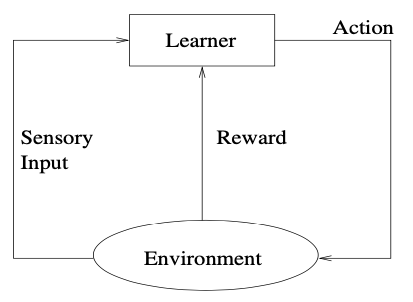
\includegraphics[width=0.35\linewidth]{rf_bp.png}
  \end{figure}
  
  \bigskip % Vertical whitespace
  
\end{frame}

\begin{frame}

  La acción puede provocar un cambio en el entorno del agente, afectando así las opciones y acciones futuras del agente. Los efectos de las acciones sobre el medio ambiente y los estados futuros no siempre se pueden predecir. Por lo tanto, es necesario que el agente monitoree frecuentemente su entorno.

  \bigskip % Vertical whitespace

  El Aprendizaje por refuerzo tiene dos importantes componentes:
  
  \begin{enumerate}
  \item Una búsqueda de prueba y error para encontrar buenas acciones, que forma el componente de exploración de Aprendizaje por Refuerzo.
  \item Un recuerdo de qué acciones funcionaron bien en qué situaciones. Este es el componente de explotación de Aprendizaje por Refuerzo.
  \end{enumerate}
\end{frame}

\begin{frame}
  
  Un agente de aprendizaje por refuerzo tiene los siguientes componentes:

  \bigskip % Vertical whitespace
  
  \begin{enumerate}
  \item \textbf{Una política}, que es la función de toma de decisiones del agente. 
  \item \textbf{Una función de recompensa}, que define el objetivo del agente.
  \item \textbf{Una función de valor}, que especifica el objetivo a largo plazo.
  \item Opcionalmente, un agente de aprendizaje reforzado también puede tener un \textbf{modelo del entorno.}
  \end{enumerate}
      
\end{frame}

\begin{frame}

  Se han propuesto varios modelos:

  \begin{enumerate}
  \item \textbf{finite-horizon model}, en el que el agente optimiza su recompensa esperada para los siguientes $n_t$ pasos, es decir \[ E \left[ \sum_{t=1} ^{n_{t}} r(t) \right]\]
  \item \textbf{infinite-horizon discounted model}, que toma en consideración toda la recompensa a largo plazo del agente. Sin embargo, cada recompensa recibida en el futuro se descuenta geométricamente de acuerdo con un factor de descuento, $\gamma \in [0, 1)$: \[ E \left[ \sum_{t=0} ^{\infty} \gamma^{t} r(t) \right]\]
  \item \textbf{average reward model}, que prefiere acciones que optimicen la recompensa promedio a largo plazo del agente: \[ \lim_{n_{t}\to\infty} E \left[ \frac{1}{n_{t}}\sum_{t=0} ^{\infty} r(t) \right]\]
  \end{enumerate}
  
\end{frame}

\begin{frame}

  \frametitle{Modelo de aprendizaje por refuerzo sin modelo}

  El objetivo es obtener una póliza óptima sin un modelo del entorno

  \bigskip % Vertical whitespace
  
  \textbf{Aprendizaje de diferencias temporales}, aprende la política de valor usando la regla de actualización

  \[ V(s) = V(s) + \eta (r+\gamma V(s') - V(s))\]

  donde $\eta$ es una tasa de aprendizaje, $r$ es la recompensa inmediata, $\gamma$ es el factor de descuento, $s$ es la estado actual, y $s$ es un estado futuro. Con base en la ecuación, siempre que un estado, $s$, se visita, su valor estimado se actualiza para estar más cerca de $r + \eta V(s')$
  
\end{frame}

\begin{frame}

  \frametitle{Q-Learning}

  la tarea es aprender los valores de refuerzo descontados esperados, $Q(s,a)$, de realizar la acción $a$ en el estado $s$, y luego continuar eligiendo siempre las acciones de manera óptima. Para relacionar los valores $Q$ con la función de valor, tenga en cuenta que \[ V*(s) = max Q*(s,a)\]

  Donde $V*(s)$ es el valor de $s$ asumiendo que la mejor acción se toma inicialmente

  \bigskip % Vertical whitespace
  
  La regla de Q-learning se da como\\

  \[ Q(s,a) = Q(s,a) + \eta(r+\gamma max Q(s',a') - Q(s,a))\]

  Luego, el agente realiza la acción con el valor $Q$ más alto.
  
\end{frame}

\section{Redes neuronales y aprendizaje por refuerzo}
\begin{frame}
  \frametitle{Redes neuronales y aprendizaje por refuerzo}

  Las redes neuronales y el aprendizaje por refuerzo se han combinado de varias maneras. Un enfoque para combinar estos modelos es utilizar un NN como aproximador de la función de valor utilizada para predecir la recompensa futur. Otro enfoque utiliza RL para ajustar los pesos

  \bigskip % Vertical whitespace

  Otros enfoques para usar RL para el entrenamiento de NN incluyen RPROP y el descenso de gradiente en la recompensa esperada. El Q-learning conexionista se utiliza para aproximar la función de valor.
  
\end{frame}

\begin{frame}
  \frametitle{RPROP}

  La propagación resiliente (RPROP) realiza una adaptación directa del peso paso usando información de gradiente local. Los ajustes de peso se implementan en el forma de recompensa o castigo, como sigue:

  \bigskip

  Si la derivada parcial, $\frac{\partial E}{\partial v_{ji}}$ (o $\frac{\partial E}{\partial w_{kj}}$) de peso $v_{ji}$ (o $w_{kj}$) cambia de signo, el valor de actualización del peso, $\Delta_{ji}$ ($\Delta_{kj}$), se reduce por el factor, $\eta^{-}$. El motivo de esta penalización es que la última actualización de peso fue demasiado grande, lo que provocó que el algoritmo saltara por encima de un mínimo local. Por otro lado, si la derivada conserva su signo, el valor de actualización se incrementa por el factor $\eta^{+}$ para acelerar la convergencia.
  
\end{frame}

%------------------------------------------------
\begin{frame}
  
  \begin{figure}
    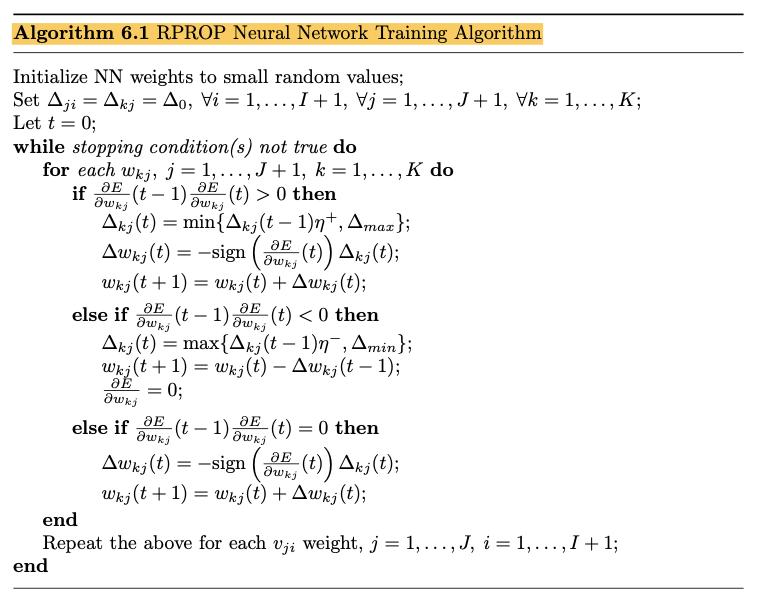
\includegraphics[width=0.98\linewidth]{rprop.png}
  \end{figure}
  
\end{frame}
%------------------------------------------------

\begin{frame}
  \frametitle{Aprendizaje por refuerzo de descenso de gradiente}

  Para problemas en los que solo se maximiza la recompensa inmediata (es decir, no hay una función de valor, solo una función de recompensa), Williams propuso reglas de actualización de peso que realizan un descenso de gradiente en la recompensa esperada. Estas reglas se integran luego con la propagación hacia atrás. Los pesos se actualizan de la siguiente manera:\\

  \[\Delta w_{kj} = \eta_{kj} (r_{p} - \Theta_{k})e_{kj}\]
\end{frame}

\begin{frame}
  
  Donde $\eta_{kj}$ es un rango de aprendizaje no negativo, $r_{p}$ es el reforzamiento asociado con el patrón $z_{p}$, $\Theta_{k}$ es el valor umbral de refuerzo, y $e_{kj}$ es la elegibilidad del peso $w_{kj}$, dado como

  \[ e_{kj} = \frac{\partial}{\partial w_{kj} [ln(g_{j}]}\]

  donde: $g_{j}=P(o_{k,p} = t_{k,p} | w_{k},z_{p}$ es la función de densidad de probabilidad utilizada para generar acciones aleatoriamente, en función de si el objetivo se predijo correctamente o no.
\end{frame}

\begin{frame}
  \frametitle{Q-Learning conexionista}

  El NN se utiliza para aproximar el mapeo entre estados y acciones, e incluso para generalizar entre estados. La entrada a la NN es el estado actual del entorno y la salida representa la acción a ejecutar. Si hay na acciones, entonces se puede usar un NN con na unidades de salida, o $n_a$ NN, uno para cada una de las acciones, se puede usar
  
\end{frame}

\begin{frame}
  \begin{figure}
    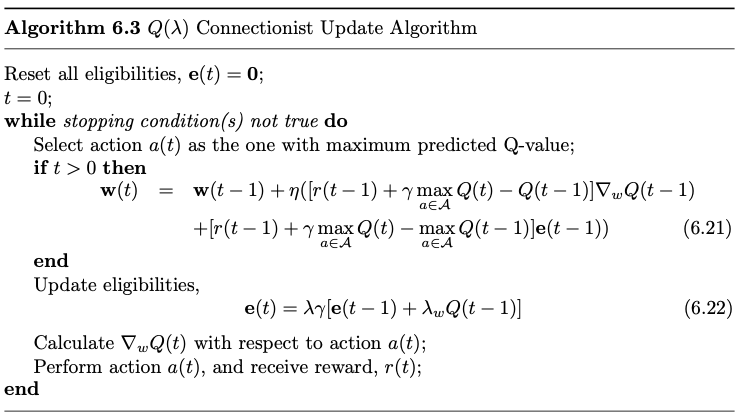
\includegraphics[width=0.98\linewidth]{connectionist_q.png}
  \end{figure}
\end{frame}

\begin{frame}
  \begin{figure}
    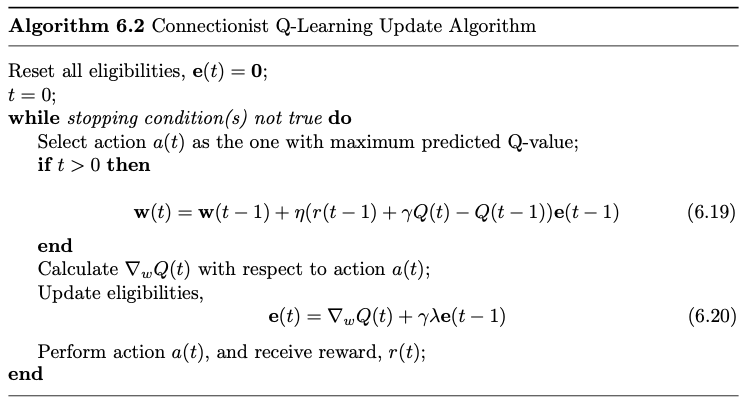
\includegraphics[width=0.98\linewidth]{connectionist_update.png}
  \end{figure}
\end{frame}

%------------------------------------------------


\end{document} 
